\documentclass[11pt]{article}
\usepackage[margin=1in]{geometry}
\usepackage{amsmath,graphicx,booktabs,amssymb,xcolor,hyperref,listings}
\usepackage[skip=4pt]{caption}
\hypersetup{colorlinks=true,linkcolor=blue!55!black,urlcolor=blue!55!black}
\newcommand{\fig}[1]{\includegraphics[width=\linewidth]{figs/#1}}
\newcommand{\good}[1]{\textcolor{green!45!black}{#1}}
\newcommand{\bad}[1]{\textcolor{red!70!black}{#1}}
\lstset{basicstyle=\ttfamily\footnotesize,breaklines=true,frame=single,framerule=0.3pt,
        xleftmargin=6pt,framexleftmargin=6pt,commentstyle=\color{gray}}
\sloppy
\title{\textbf{An implementation note on HCAPO:}\\[2pt]
\large how a wrong $\rho$ denominator manufactured a length runaway ---\\
and why the paper-correct form ignites one too}
\author{Agentic-RL-CA project}
\date{2026-07-29, updated 2026-07-30 (step-200 falsification)}

\begin{document}
\maketitle

\begin{abstract}
\noindent While ablating HCAPO (arXiv:2603.08754) on SearchQA (Qwen3-4B, non-thinking, 2048-token
response cap), our runs reproduced a severe response-length runaway --- mean length inflating
$15\times$ (89$\to$1642 tokens/turn) with 78\% of turns clipping at the cap --- while accuracy stayed
flat. Per-turn instrumentation of the hindsight ratio $\rho$ traced the cause to a single line:
\textbf{our port divided by the on-policy probability of the action, where the paper divides by the
intra-trajectory mean of the hindsight probabilities} (Eq.~7). The wrong ratio is systematically
$<1$ and, because only its numerator saturates with response length while the $1/n_{tok}$
normalisation keeps growing, it \emph{rewards verbosity}: emitting more tokens mechanically raises
$\rho$, hence the advantage. We derive the mechanism, verify it in a controlled synthetic test
(legacy $\rho$ moves $+0.13$ when responses lengthen $16\to64$ tokens; the paper form moves $0.0$),
and show the corrected implementation restores every property the paper assumes: $\rho$ centred on
$1.0$, two-sided, and discriminating between turns for the first $\sim$150 steps.
\textbf{Update (step 200): the corrected run then ignited the same runaway}
($221\to1232$ tokens between steps 150 and 200, clip $0.51$) --- falsifying our structural
prediction. The $\rho$ instrumentation identifies the shared root: Eq.~6's \emph{per-token-mean}
scoring is pulled toward generic fluency as turns lengthen, so a below-mean turn can raise its
$\rho$ by lengthening; the intra-trajectory normalisation cancels uniform inflation but not this
transient, and the across-turn spread collapses ($\sigma$: $0.135\to0.030$) until the hindsight
term is inert. On this task the published formulation, not merely our port of it, carries a length
instability. All prior HCAPO numbers from this codebase characterise the buggy variant; the
corrected run characterises the published method on SearchQA.
\end{abstract}

\section{The two formulas}

\textbf{What the paper specifies} (arXiv:2603.08754, Eq.~6--7). Per turn $t$ of a trajectory with
$T$ turns, with $s_{final}$ the trajectory's last observation injected into the prompt:
\begin{align}
\pi_{hind}(a_t) &= \exp\Big(\tfrac{1}{T_{temp}\,|a_t|}\textstyle\sum_j \log
\pi_\theta\big(y_j \mid y_{<j},\, s_t,\, s_{final}\big)\Big) \tag{Eq.~6}\\[2pt]
\rho_t &= \mathrm{clip}\Big(\;\pi_{hind}(a_t)\,\big/\,\overline{\pi}_{hind}\;,\;C_{min},C_{max}\Big),
\qquad \overline{\pi}_{hind}=\tfrac{1}{T}\textstyle\sum_{k=1}^{T}\pi_{hind}(a_k) \tag{Eq.~7}
\end{align}
The denominator is the \textbf{intra-trajectory mean over that trajectory's turns} --- the paper
calls it ``group-normalization across actions within the same episode''. By construction $\rho$ is
centred on $1.0$: pivotal turns score $>1$, redundant turns $<1$, and the symmetric clip
$[C_{min},C_{max}]=[0.8,1.2]$ is well-specified around that centre. $\rho$ then scales a discounted
return, $Q^H_t=\rho_t\,\gamma^{T-1-t}R$, which is group-normalised across the $G$ rollouts of the
prompt and added (weight $\omega$) to the standard GRPO term.

\medskip
\textbf{What we implemented} (\texttt{gigpo/core\_hcapo.py}, pre-2026-07-29):
\begin{lstlisting}[language=Python]
mean_logratio = ((hindsight_log_probs - policy_log_probs) * mask).sum(-1) / ntok
rho = exp(mean_logratio / t_temp).clamp(0.8, 1.2)
#   == pi_hind(a_t) / pi_POLICY(a_t)      <- divided by the ON-POLICY prob of the action
\end{lstlisting}
The numerator matches Eq.~6 exactly (per-token-normalised, temperature-sharpened hindsight
log-prob). The denominator does not: instead of comparing each turn's hindsight score against its
\emph{siblings in the same trajectory}, it compares hindsight against on-policy conditioning of the
\emph{same} tokens. That ratio measures something else entirely: \emph{how much the injected
$s_{final}$ text perturbs the model off-distribution} --- which is why, measured over 325 training
steps, our $\rho$ was \textbf{never once above $1.0$} (max $0.9986$; the upper clip literally never
bound) while $10.5\%$ of turns pinned at the $0.8$ floor.

\section{Why the wrong ratio rewards verbosity}

Write the per-token log-ratio $\delta_j=\log\pi(y_j\mid y_{<j},s,s_{final})-\log\pi(y_j\mid
y_{<j},s)$, so $\texttt{mean\_logratio}=\frac{1}{n_{tok}}\sum_j\delta_j$. If $\delta_j$ had a
position-independent mean, $n_{tok}$ would cancel and length would not matter. It does not: the
hindsight text perturbs the \emph{prompt}, and both conditionings share the identical generated
prefix $y_{<j}$, so $\delta_j$ is large (negative) on the first tokens --- where the prompt
dominates the context --- and decays toward $0$ as the response's own text takes over. The numerator
therefore \textbf{saturates} at some constant $C^-$ while the divisor grows:
\[
\texttt{mean\_logratio}\;\approx\;\frac{C^-}{n_{tok}}\;\xrightarrow{\;n_{tok}\uparrow\;}\;0^-,
\qquad\Rightarrow\qquad \rho=\exp(\texttt{mean\_logratio}/T_{temp})\;\to\;1^-.
\]
Longer responses $\Rightarrow$ higher $\rho$ $\Rightarrow$ higher $Q^H$.

Two independent confirmations:

\textbf{(a) The training data itself.} Inverting the logged $\rho$ to the implied \emph{total}
$\sum_j\delta_j = T_{temp}\ln(\rho)\,n_{tok}$: at step 25 ($n_{tok}{=}89$, $\rho{=}0.909$) the sum is
$-42.5$; at step 300 ($n_{tok}{=}1635$, $\rho{=}0.996$) it is $-36.0$. \textbf{Length grew
$18\times$; the total hindsight effect did not grow at all} (Fig.~\ref{fig:dilution}, left). The
entire rise of $\rho$ is the denominator. (Order-of-magnitude arithmetic: early values are censored
by the $0.8$ clip floor, and inverting a batch mean through $\exp$ is Jensen-approximate.)

\textbf{(b) A controlled synthetic test.} Fix a front-loaded perturbation ($\delta_j=-2$ on the
first 8 tokens, $0$ after) and vary only response length (Fig.~\ref{fig:synthetic}): the legacy
$\rho$ climbs from $0.82$ toward $1.0$ as $n_{tok}$ grows ($+0.13$ between 16 and 64 tokens); the
paper's $\rho$ is \textbf{exactly length-invariant} --- numerator and denominator share the same
per-token-normalised functional form, so any uniform length change cancels. Note this immunity does
\emph{not} depend on the front-loading diagnosis being right, which is a good property.

\begin{figure}[h]\centering\fig{fig_dilution.pdf}
\caption{\textbf{The dilution mechanism, measured.} \emph{Left:} in the legacy $\omega{=}1$ run, the
implied total hindsight log-ratio $\sum_j\delta_j$ (red) is $\sim$flat while response length (blue)
grows $18\times$ --- $\rho$ rises purely because the $1/n_{tok}$ divisor grows. \emph{Right:} batch-mean
$\rho$ against response length: the two legacy runs trace a tight monotone curve toward $1.0$; the
paper-correct run sits at $\rho\approx1$ independent of length.}
\label{fig:dilution}
\end{figure}

\begin{figure}[h]\centering
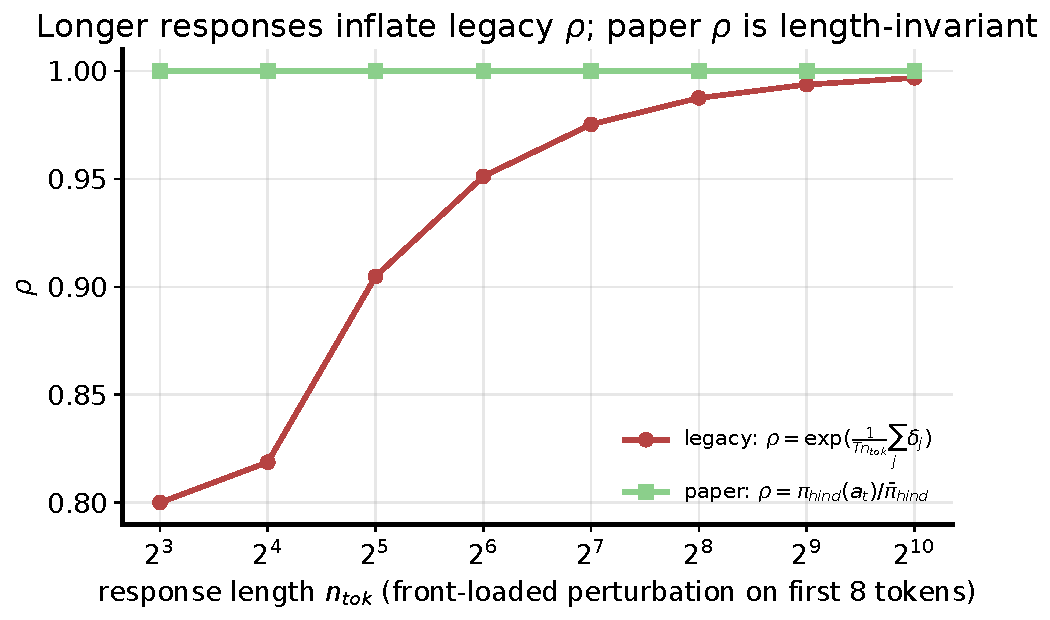
\includegraphics[width=0.62\linewidth]{figs/fig_synthetic.pdf}
\caption{\textbf{Controlled test of the mechanism.} Front-loaded perturbation ($\delta=-2$ on the
first 8 tokens), response length varied, nothing else. Legacy $\rho$ (red) inflates with length;
the paper's self-normalised $\rho$ (green) is exactly $1$ at every length.}
\label{fig:synthetic}
\end{figure}

\textbf{How a $\rho$ bias becomes a length ratchet.} $Q^H$ feeds a group normalisation across the
$G{=}5$ rollouts of each prompt, which is invariant to uniform scaling --- so ``everyone gets
longer, everyone gains'' cancels. The gradient pressure is \emph{relative}: among sibling rollouts
of the same prompt, the \textbf{longer rollout has higher $\rho$ than its siblings}, out-scores
them, and is reinforced. Each iteration the whole group lengthens, but the relative pressure
persists --- a ratchet. This predicts both observed dynamics (Fig.~\ref{fig:runaway}): a
\emph{phase transition} rather than smooth drift (legacy A: $551\to1371$ tokens in 25 steps once
the loop won), and \emph{self-termination} as $\rho$ approaches its ceiling and the across-sibling
spread compresses (legacy A: $\rho$ std $0.055\to0.038$; length plateaus at $\sim$1635 against the
2048 cap, clip $0.77$--$0.78$, \emph{above} the 0.754 that accompanied the 1.7B thinking-mode
collapse). Halving the hindsight weight ($\omega{=}0.5$, legacy B) shrinks the step size along the
same gradient --- it \textbf{delays the runaway by $\sim$125 steps but does not prevent it}.
Throughout, accuracy stayed flat ($\approx$0.39 macro-EM): the verbosity was \emph{waste}, not fuel.

\begin{figure}[h]\centering\fig{fig_runaway.pdf}
\caption{\textbf{The runaway, and its absence so far under the fix.} Mean response length (left)
and cap-clip fraction (right) per training step. Legacy $\omega{=}1$ (red) undergoes a phase
transition at $\sim$step 160 and saturates against the 2048 cap; $\omega{=}0.5$ (orange) follows the
same path $\sim$125 steps later; the paper-correct run (green) holds normal length for $\sim$150 steps --- then ignites the same
phase transition $\sim$40 steps after legacy A, reaching 1232 tokens by step 200.}
\label{fig:runaway}
\end{figure}

\section{The corrected implementation}

\texttt{gigpo/core\_hcapo.py} now implements Eq.~6--7 as the default
(\texttt{rho\_denominator="intra\_traj\_mean"}; the buggy path is retained under
\texttt{"on\_policy"} solely to reproduce the withdrawn runs):
\begin{lstlisting}[language=Python]
# Eq. 6: per-token-normalised, temperature-sharpened hindsight log-prob
log_pi_hind = (hindsight_log_probs * mask).sum(-1) / ntok / t_temp
# Eq. 7: self-normalise by the mean over the TURNS of the same trajectory
for tu in unique(traj_uid):
    idx = rows_of(tu); rep = one_row_per_distinct_turn(idx)
    xm  = log_pi_hind[rep].max()                      # numerical stability shift
    rho[idx] = exp(log_pi_hind[idx] - xm) / mean(exp(log_pi_hind[rep] - xm))
rho = clip(rho, 0.8, 1.2)
\end{lstlisting}
The policy log-probs no longer enter $\rho$ at all, matching the paper. Unit tests: (i) the
synthetic length test above (legacy $+0.1325$, paper $0.0000$); (ii) $\rho$ centred on $1.0$ with
two-sided spread on toy trajectories.

\section{The corrected form: 150 clean steps, then the same runaway}

\textbf{The structural argument we made --- and where it fails.} We argued the ratchet needs a way
for a rollout to gain by being globally more verbose, and that Eq.~7 removes it: numerator and
denominator share the $1/|a|$ normalisation, so \emph{uniform} verbosity cancels identically. That
argument is correct as far as it goes --- and was \textbf{falsified at step 200} because the
gradient it ignores is the \emph{transient, non-uniform} one. Eq.~6 scores a turn by its
\emph{per-token mean} log-prob, and a long turn's mean is dominated by generically-predictable
continuation tokens. A turn currently \emph{below} its trajectory's mean can therefore raise its
$\rho$ simply by lengthening --- diluting its distinctive (low-probability) early tokens toward
generic fluency. Lengthening is never uniform while this is happening, so the intra-trajectory
normalisation does not cancel it; the process self-terminates only when all turns have homogenised
($\rho\approx1$ everywhere) and the hindsight signal is dead.

\textbf{Empirical.} The first $\sim$150 steps looked exactly as the paper intends (single seed;
per-step instrumentation):
\begin{center}\small
\begin{tabular}{lcc}
\toprule
& legacy (withdrawn), step 1 & \textbf{paper-correct, step 1}\\
\midrule
$\rho$ mean            & 0.9078 & \good{1.0006}\\
$\rho$ min / max       & 0.800 / 0.9986 & 0.800 / \good{1.2000}\\
frac at lower clip     & 0.105 & 0.023\\
frac at upper clip     & \bad{0.000} & \good{0.014}\\
$|$macro$|$ : $|$micro$|$ (adv.\ terms) & 1 : 1.40 & 1 : 1.14\\
\bottomrule
\end{tabular}
\end{center}
Every property the paper assumes is restored: $\rho$ is centred on $1.0$ and \textbf{two-sided ---
the upper clip binds for the first time in this codebase} (1.4\% of turns), i.e.\ some turns are now
scored as \emph{pivotal}, which is the entire point of hindsight credit and was structurally
impossible under the legacy ratio. The spread is \emph{growing} (std $0.073\to0.143$ over 45 steps)
where the legacy spread collapsed ($0.055\to0.038$): the signal differentiates turns instead of
saturating (Fig.~\ref{fig:rho}). Behaviourally, at step 25: macro-EM $0.352$, clip $0.001$, response
length $91$ tokens --- indistinguishable from GRPO at the same point, as expected.

\begin{figure}[h]\centering\fig{fig_rho.pdf}
\caption{\textbf{$\rho$ statistics per training step.} \emph{Left:} legacy $\rho$ (red/orange)
starts at $0.91$ and is crushed toward $1.0$ from below as length inflates; the paper-correct run
(green) sits at $1.0$ from step one. \emph{Right:} legacy spread collapses as $\rho$ saturates toward $1$ from below; the corrected
spread grows for $\sim$100 steps (discriminating between turns) and then \emph{also} collapses
($0.135\to0.030$) as lengthening homogenises the per-token means --- the spread, not the mean, is
where the corrected form's runaway is visible.}
\label{fig:rho}
\end{figure}

\textbf{Then the ignition.} Length: $147@100 \to 221@150 \to 249@160 \to 412@170 \to 611@180
\to 985@190 \to \mathbf{1232@200}$ (clip $0.505$); EM flat across it ($0.401\to0.417\to0.408$) ---
the same phase-transition-then-waste signature as the legacy runs, $\sim$40 steps later than legacy
A. Concurrently the $\rho$ spread \emph{collapsed} ($\sigma$: $0.135@100 \to 0.068@150 \to
0.030@200$, both clip fractions $\to0$): by step 200 every turn scores $\rho\approx1$ and the
hindsight term is inert --- HCAPO has degenerated to GRPO plus a positional discount
$\gamma^{T-1-t}$, at $8\times$ GRPO's token cost. \emph{Interpretation caveats:} single seed;
SearchQA trajectories have $T\le4$ turns (a noisy 4-sample mean in Eq.~7) and our $s_{final}$ is a
long retrieved-documents block --- the paper's own tasks (ALFWorld/WebShop: short action-style
turns, 512-token caps, Qwen2.5-7B) may never enter this regime, so this is a statement about the
formulation \emph{on this task class}, not a refutation of the paper's results. The decisive
within-batch probe --- per-sample $\mathrm{corr}(\rho, |a_t|)$ before vs during ignition --- is now
the top instrumentation priority. The run continues to 500 (abort rule requires EM $<0.30$; it is
$0.408$); final update at 500.

\section{Record}
Withdrawn: both legacy 4B runs (killed at steps $\sim$324/330), and all earlier HCAPO numbers from
this codebase --- SearchQA 1.7B (0.357 @ clip 0.754), 4B legacy arms ($\approx$0.39), AlfWorld 1.7B
(0.791) --- as characterisations of the \emph{published} method (they remain valid measurements of
the buggy variant). The full timestamped trail (pre-registration, amendments, retraction of two
premature trend calls, and this correction) is in
\texttt{docs/reports/2026-07-21\_4b\_horizon\_eval/results/hcapo\_wave3\_preregistration.md}.
Provenance caveat: Eq.~6--7 were transcribed from the arXiv HTML via automated fetch (re-queried
twice, quoted verbatim); confirm against the PDF before external use. Rebuild:
\texttt{assets/build\_figures.py} (parses the three training logs directly), then
\texttt{tectonic report.tex}.
\end{document}
